\documentclass[12pt]{article}

\usepackage{amsmath,amsthm,amssymb}
\usepackage{tikz}

\newcommand{\A}{\mathcal{A}}
\newcommand{\G}{\mathcal{G}}
\renewcommand{\P}{\mathfrak{A}}
\newcommand{\C}{\mathfrak{C}}
\newcommand{\Z}{\mathbb{Z}}
\newcommand{\Q}{\mathbb{Q}}
\newcommand{\2}{\textbf{2}}
\newcommand{\Am}{\textbf{A}}
\newcommand{\del}{\partial}
\renewcommand{\v}{\bar{v}}
\newcommand{\e}{\bar{e}}
\newcommand{\T}{\mathcal{T}}

\newtheorem{thm}{Theorem}

\title{Extensions of Abelian Automata Groups}
\author{Chris Grossack}

\begin{document}
\maketitle

\section{Background}

\subsection{Mealy Automata}
Recall a \textbf{Mealy Automaton} is a combinatorial object which defines
functions from $\Sigma^* \to \Sigma^*$ for some alphabet $\Sigma$
(As usual, $\Sigma^*$ denotes the free monoid generated by $\Sigma$).
In the special case each of these functions is invertible, we say the
Automaton is an \textbf{Invertible Transducer}. For our purposes, 
a Mealey Automaton is a tuple 
$\A = (S, \Sigma, \delta)$
where $S$ is the \textbf{State Set}, $\Sigma$ is the \textbf{Alphabet},
and $\delta~:~S \times \Sigma \to S \times \Sigma$ is the
\textbf{transition function}.

Given a state $s \in S$, we can treat it is a function 
$\underline{s} : \Sigma^* \to \Sigma^*$ by 

\begin{align*}
  \underline{s}(\varepsilon) &= \varepsilon\\
  \underline{s}(ax)       &= a' \underline{s'}(x) 
  ~~~(\text{where } (s', a') = \delta(s,a))
\end{align*}
Where juxtaposition is concatenation, and $\varepsilon$ is
the identity in $\Sigma^*$.
Clearly we could treat $\underline{s}$ as a function on $\Sigma^\omega$ 
instead, and in fact we occasionally will, however we will be 
clear when doing so.

In general, one can look at the semigroup generated by an automaton $\A$,
namely the semigroup generated by $\{ \underline{s}~|~s \in S \}$.
For the rest of the paper, however, we will restrict ourselves to the
invertible case, and will consider $\G(\A)$, the group generated by 
$\{ \underline{s}~|~s \in S \}$ instead.

As an example, consider the automaton (shown below)
$\A = (\{ \alpha, \tau \}, \2, \delta)$
with 
\begin{align*}
  \delta(\alpha,0) &= (\alpha,1)\\
  \delta(\alpha,1) &= (\tau,0)\\
  \delta(\tau,0)   &= (\alpha,0)\\
  \delta(\tau,1)   &= (\tau,1)
\end{align*}

TODO: is this correct?

\begin{center}
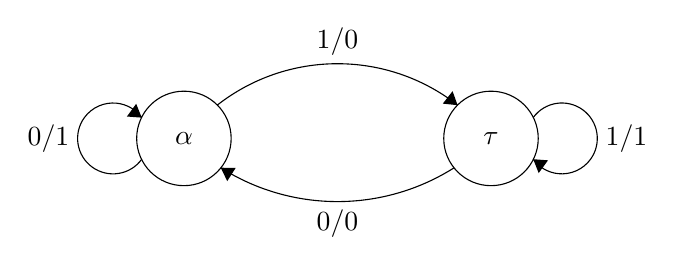
\begin{tikzpicture}[scale=0.2]
\tikzstyle{every node}+=[inner sep=0pt]
\draw [black] (15.8,-29.2) circle (3);
\draw (15.8,-29.2) node {$\alpha$};
\draw [black] (35.3,-29.2) circle (3);
\draw (35.3,-29.2) node {$\tau$};
\draw [black] (13.12,-30.523) arc (-36:-324:2.25);
\draw (8.55,-29.2) node [left] {$0/1$};
\fill [black] (13.12,-27.88) -- (12.77,-27) -- (12.18,-27.81);
\draw [black] (17.918,-27.085) arc (128.02449:51.97551:12.39);
\fill [black] (33.18,-27.09) -- (32.86,-26.2) -- (32.24,-26.99);
\draw (25.55,-23.96) node [above] {$1/0$};
\draw [black] (37.98,-27.877) arc (144:-144:2.25);
\draw (42.55,-29.2) node [right] {$1/1$};
\fill [black] (37.98,-30.52) -- (38.33,-31.4) -- (38.92,-30.59);
\draw [black] (32.957,-31.065) arc (-57.68311:-122.31689:13.856);
\fill [black] (18.14,-31.06) -- (18.55,-31.91) -- (19.09,-31.07);
\draw (25.55,-33.71) node [below] {$0/0$};
\end{tikzpicture}
\end{center}

Somewhat surprisingly, $\G(\A)$ is the lamplighter group, $\Z/2\Z \wr \Z$

\subsection{Abelian Automata}
We restrict ourselves to the case where $\G(\A)$ is abelian, 
and use methods of Nekrashevich and Sidki to characterize these groups.
Further, we can take some combinatorial information from our Mealy 
Automaton, and push it into the group theoretic world. This will give
rise to much of the interesting structure of these groups, since
$\G(\A)$ is abelian if and only if it is either free abelian or 
boolean.

It is well known that in an Invertible Transducer, each $\delta(s,-)$
is a permutation of $\Sigma$. Since our automata will be over the alphabet
\2, this means every state either flips its input 
(in which case it is called an \textbf{Odd} or \textbf{Toggle State}), 
or does not
(in which case it is called an \textbf{Even} or \textbf{Copy State}).
We extend these definitions to the entire group, and say $f \in \G(\A)$ 
is odd iff it flips the first bit of its input.

Further, recall the \textbf{0-residual} (resp. \textbf{1-residual}) of a 
function $f \in \G(\A)$ is the unique function 
$\del_0 f$ such that $f(0w) = f(0) \del_0 f(w)$ 
(resp. $f(1w) = f(1) \del_1 f(w)$). 
For a state $s \in \A$, it is clear that 
$\del_i \underline{s} = \underline{\delta(s,i)}$.

It is a theorem by Sutner that $\G(\A)$ is abelian iff for 
even states $\del_0 f - \del_1 f = I$ and for odd states
$\del_1 f - \del_0 f = \gamma$, where $\gamma$ is independent
of $f$. Here we write $I$ for the identity element of our group,
and we use additive notation since our groups are abelian.

Further, the case $\gamma = I$ corresponds precisely to the $\G(\A)$
being boolean.

We now restrict ourselves further to the case where $\G(\A)$ is 
free abelian, that is to say $\G(\A) \cong \Z^m$ for some $m$,
and $\gamma \not = I$.
If $\varphi$ witnesses this isomorphism, then $\varphi(f)$ has odd
first component iff $f$ is odd. To that end, we call a vector $\v$ odd
if its first component is odd, and even otherwise.

A theorem by Nekrashevich and Sidki tells us that

\begin{thm}[Nekrashevich and Sidki]
  There is a matrix $\Am$ associated to each automaton 
  (though multiple automata may share a matrix, as we will soon see)
  such that for any odd vector $\e$ 
  \[ \del_0 f = \Am (\varphi(f) - \e) \] and
  \[ \del_1 f = \Am (\varphi(f) + \e) \]

  For even vectors, 
  \[ \del_0 f = \del_1 f = \Am (\varphi(f)) \]
  Futher, $\Am$ is a contraction (all its complex eigenvalues have norm $<1$),
  and $\Am$ has irreducible characteristic polynomial 
  $\chi(x) = x^m + \frac{1}{2}g(x)$, 
  where $g \in \Z[x]$ has constant term $\pm 1$
\end{thm}

To that end, we can define the \textbf{Complete Automaton} 
$\mathfrak{C}(\Am, \e)$ as the Mealy machine whose state set is all of
$\Z^m$, and whose transitions are given by the above formulas.

Notice that we can take any state $f \in \mathfrak{C}(\Am, \e)$, 
and close $\{ f \}$ under residuation.
Further, since $\Am$ is a contraction, the resulting closure will be finite.
We call this machine $\A_f$, and recognize $\G(\A_f)$ is a subgroup of 
$\G(\mathfrak{C}(\Am, \e))$.

The free parameter $\e$ seems confusing at first. Particularly 
when one tries to understand how it effects the $\A_f$ which live in
$\mathfrak{C}(\Am, \e)$. We will show later that every abelian automaton
lives in $\mathfrak{C}(\Am, \e)$ for infinitely many $\e$, and
further we will characterize exactly which $\e$ these are, and for which
$f$ is $\A_f \subseteq \mathfrak{C}(\Am, \e)$ the desired automaton.

To that end, we will say that a function $f$ is \textbf{Located at} 
$\v \in \mathfrak{C}(\Am, \e)$ iff some isomorphism $\varphi$ sends 
$f$ to $\v$. We make an analogous definition for an entire automaton $\A$
being \textbf{Located at} $f$ if 
$\A = \A_f \subseteq \mathfrak{C}(\Am, \e)$

\subsection{Principal Automata}
It was shown by Okano that there is a distinguished automaton $\P$, 
called the \textbf{Principal Automaton}, associated to each matrix.
$\P$ is defined to be 
$\P = \A_{\e_1} \cup \A_{-\e_1} \subseteq \mathfrak{C}(\Am, \e_1)$,
though there is a longstanding conjecture that in most cases this is
the same machine as
$\A_{\e_1} \subseteq \mathfrak{C}(\Am, \e_1)$.

Let us now collect a few facts about the principal automaton.

Let $\delta = \e_1 \in \mathfrak{C}(\Am, \e_1)$ 
denote the generator for $\P$. We will show soon
that $\P$ is located at $\e \in \mathfrak{C}(\Am, \e)$ for all odd $\e$,
and so calling it $\delta$ will remove ambiguity in the future.

Further, notice that $\del_0 \delta = \Am(\e_1 - \e_1) = \bar{0}$, 
the identity function. 
Then $\gamma = \del_1 \delta - \del_0 \delta = \del_1 \delta$.

Additionally, $\P$ is minimal in the following sense: 
$\G(\P) \leq \G(\A)$ for every $\A$ sharing a matrix with $\P$. 
While there are proofs of this claim which rely heavily on the
ambient linear algebraic structure, we present here a construction
which uses only the given automaton $\A$ to construct $\P$.

In fact, it is easy to see that $\P$ will be located at $\e$ in
$\mathfrak{C}(\Am, \e)$ for all $\e$. A proof has been
omitted, as we will prove a much more general version of this claim
in the next section.

\begin{proof}
  Let $\A$ be an abelian automaton with at least one odd state.
  Note that if $\A$ has no odd states, its group is trivial, 
  and therefore any principal machine can be associated to it.

  Put $\gamma = \del_1 f - \del_0 f$ for $f \in \A$ odd, and construct
  a new automaton by closing $\gamma$ under residuation.

  Note that this can be done using only information contained in $\A$,
  since it is well known that:
  \[
    \del_0(f + g) = \begin{cases} \del_0 f + \del_1 g & \text{both odd}\\
                                  \del_0 f + \del_0 g & \text{otherwise}
                    \end{cases}
  \]
  \[
    \del_1(f + g) = \begin{cases} \del_1 f + \del_0 g & \text{both odd}\\
                                  \del_1 f + \del_1 g & \text{otherwise}
                    \end{cases}
  \]
  \[
    \del_0 (-f) = - \del_1 f
  \]
  \[
    \del_1 (-f) = - \del_0 f
  \]

  Thus using the characterization by Sutner that a state is odd iff it has 
  distinct residuals, we can close $\gamma$ under residuation by looking
  only at $\A$.

  Now, if necessary, we can join this automaton with its negation, and
  possibly add states $\delta$ and $-\delta$ residuating into $I$
  (an even self loop) and $\pm \gamma$
\end{proof}

\subsection{An Example}
Consider the following machine, which will show up again in section ??.

\begin{center}
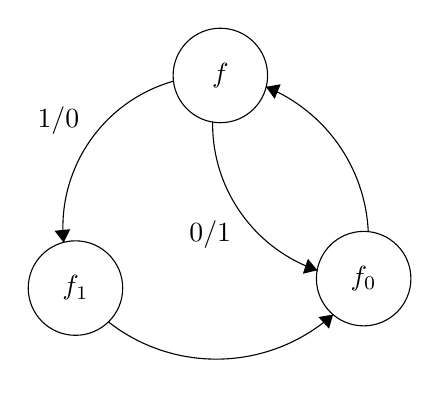
\begin{tikzpicture}[scale=0.2]
\tikzstyle{every node}+=[inner sep=0pt]
\draw [black] (26.6,-12.1) circle (3);
\draw (26.6,-12.1) node {$f$};
\draw [black] (17.4,-25.6) circle (3);
\draw (17.4,-25.6) node {$f_1$};
\draw [black] (35.7,-25) circle (3);
\draw (35.7,-25) node {$f_0$};
\draw [black] (16.648,-22.708) arc (-174.31762:-254.2298:9.658);
\fill [black] (16.65,-22.71) -- (17.07,-21.86) -- (16.07,-21.96);
\draw (17.67,-14.97) node [left] {$1/0$};
\draw [black] (33.761,-27.277) arc (-48.14861:-128.09563:11.117);
\fill [black] (33.76,-27.28) -- (32.83,-27.44) -- (33.5,-28.18);
\draw [black] (29.501,-12.822) arc (67.8011:2.5992:10.451);
\fill [black] (29.5,-12.82) -- (30.05,-13.59) -- (30.43,-12.66);
\draw [black] (32.758,-24.474) arc (-108.88288:-180.71682:9.832);
\fill [black] (32.76,-24.47) -- (32.16,-23.74) -- (31.84,-24.69);
\draw (27.31,-22.21) node [left] {$0/1$};
\end{tikzpicture}
\end{center}

Here the unlabeled transitions both copy the input bit, however these
have been omitted for cleanliness.

Then we can construct the principal machine as follows:

\begin{center}
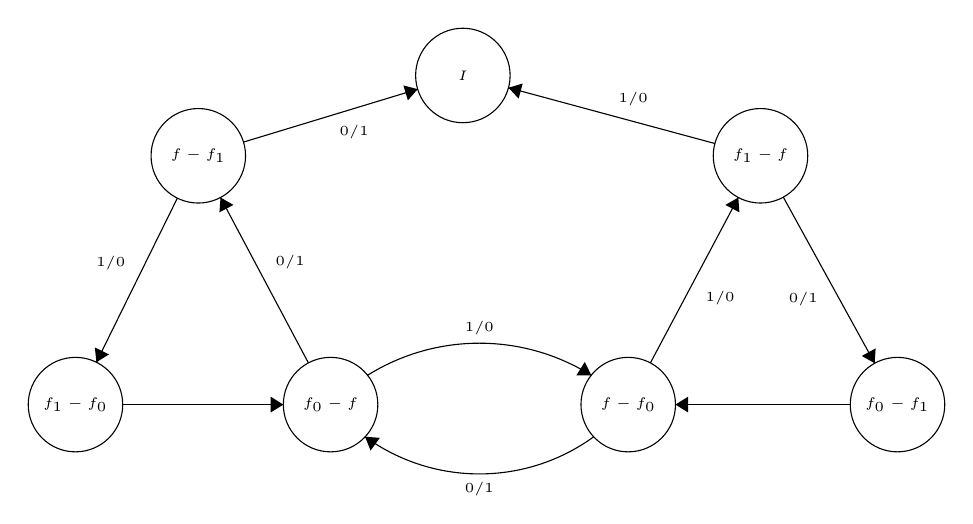
\begin{tikzpicture}[scale=0.2]
\tikzstyle{every node}+=[inner sep=0pt]
\draw [black] (36.4,-15.9) circle (3);
\draw (36.4,-15.9) node {\tiny $I$};
\draw [black] (55.3,-21) circle (3);
\draw (55.3,-21) node {\tiny $f_1-f$};
\draw [black] (64,-36.8) circle (3);
\draw (64,-36.8) node {\tiny $f_0-f_1$};
\draw [black] (46.9,-36.8) circle (3);
\draw (46.9,-36.8) node {\tiny $f-f_0$};
\draw [black] (28,-36.8) circle (3);
\draw (28,-36.8) node {\tiny $f_0-f$};
\draw [black] (11.8,-36.8) circle (3);
\draw (11.8,-36.8) node {\tiny $f_1-f_0$};
\draw [black] (19.6,-21) circle (3);
\draw (19.6,-21) node {\tiny $f-f_1$};
\draw [black] (22.47,-20.13) -- (33.53,-16.77);
\fill [black] (33.53,-16.77) -- (32.62,-16.53) -- (32.91,-17.48);
\draw (29.5,-19.03) node [below] {\tiny $0/1$};
\draw [black] (18.27,-23.69) -- (13.13,-34.11);
\fill [black] (13.13,-34.11) -- (13.93,-33.61) -- (13.03,-33.17);
\draw (15,-27.81) node [left] {\tiny $1/0$};
\draw [black] (14.8,-36.8) -- (25,-36.8);
\fill [black] (25,-36.8) -- (24.2,-36.3) -- (24.2,-37.3);
\draw [black] (26.59,-34.15) -- (21.01,-23.65);
\fill [black] (21.01,-23.65) -- (20.94,-24.59) -- (21.83,-24.12);
\draw (24.48,-27.74) node [right] {\tiny $0/1$};
\draw [black] (30.345,-34.939) arc (122.03013:57.96987:13.397);
\fill [black] (44.56,-34.94) -- (44.14,-34.09) -- (43.61,-34.94);
\draw (37.45,-32.4) node [above] {\tiny $1/0$};
\draw [black] (52.4,-20.22) -- (39.3,-16.68);
\fill [black] (39.3,-16.68) -- (39.94,-17.37) -- (40.2,-16.41);
\draw (47.22,-17.84) node [above] {\tiny $1/0$};
\draw [black] (56.75,-23.63) -- (62.55,-34.17);
\fill [black] (62.55,-34.17) -- (62.61,-33.23) -- (61.73,-33.71);
\draw (58.98,-30.09) node [left] {\tiny $0/1$};
\draw [black] (61,-36.8) -- (49.9,-36.8);
\fill [black] (49.9,-36.8) -- (50.7,-37.3) -- (50.7,-36.3);
\draw [black] (48.31,-34.15) -- (53.89,-23.65);
\fill [black] (53.89,-23.65) -- (53.07,-24.12) -- (53.96,-24.59);
\draw (51.78,-30.06) node [right] {\tiny $1/0$};
\draw [black] (44.711,-38.841) arc (-53.966:-126.034:12.343);
\fill [black] (30.19,-38.84) -- (30.54,-39.72) -- (31.13,-38.91);
\draw (37.45,-41.7) node [below] {\tiny $0/1$};
\end{tikzpicture}
\end{center}

It is easy to check that this is the principal machine for
$\Am = \begin{pmatrix} -1 & 1 \\ -\frac{1}{2} & 0 \end{pmatrix}$,
and further that $\A$ as above is located at 
$\e_1 \in \mathfrak{C}\left ( \Am, \begin{pmatrix} 3 \\ 2 \end{pmatrix} \right )$

Notice that in this case we did not need to explicitly add the 
inverse machine, or indeed $\pm \delta$. The Strongly Connected Component
Conjecture states that for almost all abelian automata, this will be the case.
However, this conjecture is yet unproven.

\section{Group Extensions}
Going forward, $\G$ will denote $\G(\P)$ for some principal machine $\P$.

In the case of interest, $\G \cong \Z^m$. Further, $\del_0$ extends to 
a matrix $\Am$ of irreducible character as in Thm 1. Then
$\G$ admits representation as a $\Z[x]$ module where 
$x \cdot \v = \Am^{-1}\v$, extended linearly.
Further, since $\Am$ has irreducible character (in $\Z$ and in $\Q$), 
so does $\Am^{-1}$. Thus this module is cyclic, 
and generated by $\e_1 = \delta$.

Clearly $\text{End}_{\G}$, the ring of module endomorphisms of $\G$, 
is isomorphic to $\Z[x]/(\chi^*)$, 
where $\chi^*$ is the characteristic polynomial of $\Am^{-1}$.
Now for some $p \in \text{End}_{\G}$ we write
$p \cdot \G$ in place of $\G(\mathfrak{C}(\Am,p \cdot \e_1))$.

That is to say, $p \cdot \G$ has as its states $\Z^m$ and as its 
residuations
$\del_0 \v = \Am (\v - p \cdot \e_1)$, and 
$\del_1 \v = \Am (\v + p \cdot \e_1)$

Since the residuation vector must be odd, we note $p$ must have odd
constant term.

For reasons which will soon become clear, we call $p \cdot \G$ the
\textbf{Group Extension} of $\G$ by $p$.

To justify this nomenclature, we first notice 
$\G \hookrightarrow p \cdot \G$ for all $p$ by the
homomorphism $\v \mapsto p \cdot \v$. 
Further, we recognize that if $p$ is not a unit in $\text{End}_{\G}$, 
this homomorphism is \emph{not} surjective. 
That is to say $\G$ is a proper subgroup of $p \cdot \G$.
\textbf{Note:} It \emph{is} the case that $\G \cong \Z^m \cong p \cdot \G$. 

Every function $f \in \G$ is also an element of $p \cdot \G$. 
If $f \in \G$ is located at $\v$, then $f \in p \cdot \G$ is located
at $p \cdot \v$. In fact, this is true in a more general sense:

\begin{thm}
  If $rp = q$, then $p \cdot \G \hookrightarrow q \cdot \G$, 
  with a canonical injection $\phi_r~:~\v \mapsto r \cdot \v$. 
  In particular, if $r$ is a unit, then $p \cdot \G \cong q \cdot \G$.
\end{thm}

\begin{proof}
  Let $rp = q$, $f \in p \cdot \G$ located at $\v$.
  Consider $f' \in q \cdot \G$ located at $r \cdot \v$.

  First note $f$ and $f'$ have the same parity, since 
  $r$ has odd constant term, and so $\v$ and $r \cdot \v$
  have the same parity. Now, consider the residuals of $f$ and $f'$. 
  
  If $f$ is even, then 
  \[ \del_0 f' = \Am (r \cdot \v) = r \cdot \Am \v = r \cdot \del_0 f \]

  If $f$ is odd, then
  \[ \del_0 f' = \Am (r \cdot \v - q \cdot \e_1) 
               = r \cdot \Am (\v - p \cdot \e_1)
               = r \cdot \del_0 f \]

  A similar argument shows $\del_1 f' = r \cdot \del_1 f$
\end{proof}

\section{Fractional Elements}
So for $p \cdot \G$ we know exactly how vectors of the form $p \cdot \v$
behave as functions: They are exactly the functions present in $\G$.
However there are plenty of vectors which do not have the above form. 
How do they behave? We call such vectors (and their corresponding functions)
\textbf{Fractional}, due to the following observation.

Consider $3 \cdot \G$. What does $\e_1$ do as a function?
Well, $3\e_1$ is the same function as $\delta$, and so
$\e_1$ should behave like ``$\frac{1}{3}\delta$'', and in fact it does.

In general, $\v \in p \cdot \G$ behaves like $p^{-1} \cdot \v \in \G$,
(where $p^{-1}$ comes from $\Q[x]$ and so $p^{-1} \cdot \v \in \Q^m$)
and so Group Extensions give us access to fractional functions from 
our base group $\G$.

\begin{thm}
  $\forall p \in Z[x]$ with odd constant term, 
  $p^{-1} \cdot \Z^m \cong p \cdot \G$.
  Further, this isomorphism respects $\del_0$ and $\del_1$.
\end{thm}

\begin{proof}
  Here we think of $p^{-1} \cdot \Z^m = \{ p^{-1} \cdot \v~|~\v \in \Z^m \}$
  as a subgroup of $\Q^m$. Residuaition in this setting is given by
  $\del_0 \v = \Am (\v - \e_1)$ and $\del_1 \v = \Am (\v + \e_1)$ 

  Consider $\varphi~:~p^{-1} \cdot \Z^m \to p \cdot \G$ by
  $\varphi(p^{-1} \cdot \v) = \v$.\\
  $\varphi$ is clearly bijective, and is a homomorphism since:
  \begin{align*}
       \varphi(p^{-1} \cdot \v_1 + p^{-1} \cdot \v_2) 
    &= \varphi(p^{-1} \cdot (\v_1 + \v_2))\\
    &= \v_1 + \v_2\\
    &= \varphi(p^{-1} \cdot \v_1) + \varphi(p^{-1} \cdot \v_2) 
  \end{align*}

  Further, if $\v$ is even, then:

  \begin{align*}
       \varphi(\del_0 p^{-1} \cdot \v)
    &= \varphi(\Am p^{-1} \cdot \v)\\
    &= \varphi(p^{-1} \cdot \Am \v)\\
    &= \Am \v\\
    &= \del_0 \varphi(p^{-1} \cdot \v)
  \end{align*}

  If $\v$ is odd, then: 

  \begin{align*}
       \varphi(\del_0 p^{-1} \cdot \v)
    &= \varphi(\Am (p^{-1} \cdot \v - \e_1))\\
    &= \varphi(p^{-1} \cdot \Am (\v - p \cdot \e_1))\\
    &= \Am (\v - p \cdot \e_1)\\
    &= \del_0 \varphi(p^{-1} \cdot \v)
  \end{align*}

  The proof for $\del_1$ is similar.
\end{proof}

Thus we can view functions in $p \cdot \G$ as fractions of functions in $\G$.
It is a natural question to ask which fractions are attainable in this way.

Clearly, for any $f \in \G$, we can attain $\frac{1}{k} f$ for any odd $k$.
However, fractions with even denominator are unattainable, 
even as limits of sequences of functions.
This is clear, since $\frac{1}{2}\delta$, for instance, must 
when applied twice, flip the first bit of the input. But it must itself
be even or odd. In either case, $2 \frac{1}{2} \delta$ does not flip the 
first bit, a contradiction.

\section{Characterizing Automata}
It is well known that every automaton $\A$ is a subautomaton of some
complete $\mathfrak{C}(\Am, \e)$.
Equaivalently every $\A$ is a subautomaton of some $p_e \cdot \G$.

Further, we now understand that the various choices of $\e$ correspond to
levels of fractional elements of $\P$, so there should be a minimal $\e$
(up to multiplication by units) which still has $\A$ as a subautomaton. 

Notice that if we locate $\A$ at $\e_1 \in p \cdot \G$, 
then there can be no smaller polynomial $q$ (in the division ordering)
which also places $\A$ at an integral position, because, by the above
theorems:\\ 
$\e_1 \in p \cdot \G$ is located at $p^{-1}q \cdot \e_1 \in q \cdot \G$, 
and $p^{-1}q \cdot \e_1$ is fractional.


\begin{thm}
  Every nontrivial abelian automaton $\A$ can be 
  located at $\e_1$ in $p \cdot \G$ for some $p$.
\end{thm}

\begin{proof}
  An algorithm for computing the matrix $\Am$ associated to $\A$ is
  described by Becker, and has been omitted.

  It is a theorem by Sutner that every abelian automaton residuates into
  a strongly connected component, and further that this component generates
  the same group as the entire machine. So we may, with no loss of generality,
  assume our machine is strongly connected.

  Let $f$ be an odd state in $\A$. Then at least one of $\del_0 f$ and 
  $\del_1 f$ is not equal to $f$. Then there is some nontrivial cycle
  from $f$ to itself, which we can represent by a matrix equation 
  relating $\v_f$, and $\e$. (Here $\v_f$ is where $f$ will be located, 
  and $\e$ will be the eventual residuation vector). 
  We can then rearrange this equation to obtain 
  $p_1(\Am)\v_f = p_2(\Am)\e$.

  However, $p_1, p_2 \in \Z[x]$ but $\Am$ has irreducible character over $\Z$.
  It is well known that the eigenvalues of $p(\Am)$ are precisely $p(\lambda)$
  where $\lambda$ is an eigenvalue of $\Am$, so $\Am$'s invertibility implies
  the invertibility of both $p_1$ and $p_2$. Thus

  \[ \e = p_2(\Am)^{-1}p_1(\Am)\v_f \]

  Choosing $\v_f = \e_1$ gives a value for the residuation vector $\e$,
  which (by cyclicity) gives a polynomial $p_e$ 
  such that $p_e \cdot \e_1 = \e$. Then, by construction, $\A$ is 
  a subautomaton of $p_e \cdot \G$, and is anchored with $f$ at $\e_1$.
  As desired.
\end{proof}

Then for any automaton $\A$, we can now completely characterize in
which complete machines it can be located, and at what vectors.
Simply locate $\A$ at $\e_1 \in p \cdot \G$, and then to locate it at
any odd vector $\v$, scale both sides by $p_{\v}$ to see $\A$ located at
$\v \in p_{\v} p \cdot \G$.

Further, given some polynomial $q$, $\A$ is located somewhere in $q$ 
if and only if $p \vert q$. Further, it will be located at 
$p^{-1}q \cdot e_1$.

\subsection{An Example}

Consider the following abelian automaton $\A$:

TODO: Should I Show this again? Or reference it earlier in the paper?

\begin{center}
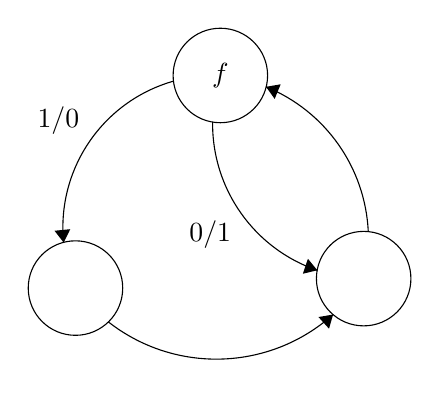
\begin{tikzpicture}[scale=0.2]
\tikzstyle{every node}+=[inner sep=0pt]
\draw [black] (26.6,-12.1) circle (3);
\draw (26.6,-12.1) node {$f$};
\draw [black] (17.4,-25.6) circle (3);
\draw [black] (35.7,-25) circle (3);
\draw [black] (16.648,-22.708) arc (-174.31762:-254.2298:9.658);
\fill [black] (16.65,-22.71) -- (17.07,-21.86) -- (16.07,-21.96);
\draw (17.67,-14.97) node [left] {$1/0$};
\draw [black] (33.761,-27.277) arc (-48.14861:-128.09563:11.117);
\fill [black] (33.76,-27.28) -- (32.83,-27.44) -- (33.5,-28.18);
\draw [black] (29.501,-12.822) arc (67.8011:2.5992:10.451);
\fill [black] (29.5,-12.82) -- (30.05,-13.59) -- (30.43,-12.66);
\draw [black] (32.758,-24.474) arc (-108.88288:-180.71682:9.832);
\fill [black] (32.76,-24.47) -- (32.16,-23.74) -- (31.84,-24.69);
\draw (27.31,-22.21) node [left] {$0/1$};
\end{tikzpicture}
\end{center}

Say we want to find $\v$ and $\e$ such that $\A$ is located at 
$\v \in \mathfrak{C}(\Am, \e)$.

Using the algorithm described by Becker gives 
$\Am = \begin{pmatrix} -1 & 1 \\ -\frac{1}{2} & 0 \end{pmatrix}$.

Then notice $\del_0 \del_0 f = f$.
So $\Am^2 (\v_f - \e) = \v_f$, and
$\Am^2 \v_f - \v_f = \Am^2 \e$. Thus

\[ \e = \Am^{-2} (\Am^2 - I) \v_f \]

Choosing $\v_f = \e_1$ gives $\e = \begin{pmatrix} 3 \\ 2 \end{pmatrix}$.

Then $f = \begin{pmatrix} 1 \\ 0 \end{pmatrix} \in (3+2x) \cdot \G$

\section{Characterizing Orbits}

Recall an \textbf{Orbit} of $f \in \G(\A)$ at $u \in \2^{\omega}$
is $\{ f^t u~|~t \in \Z \}$, or, additively, $\{ tf u~|~t \in \Z \}$.
It is a reasonable question to wonder what these orbits look like
for an arbitrary function $f$.

By the above theorem, it suffices to consider $f \in p \cdot \G$
for some principal group $\G$. Fix such a group.

We begin with a useful lemma

\begin{thm}
  $x^n \cdot \delta (u0v) = u1v$ 
  (where $|u| = n$, and $v \in \2^*$ or $\2^\omega$ arbitrary)
\end{thm}

\begin{proof}
  If $n=0$ the theorem is clear, since 
  $\delta 0v = 1 (\del_0 \delta v) = 1 (I v) = 1v$

  Further by induction, 
  $x^{n+1} \cdot \delta (u_0u0v) = 
  \Am^{-1} (x^n \cdot \delta) (u_0u0v) =
  u_0 (x^n \cdot \delta) (u0v) =
  u_0u1v$
\end{proof}

We will first prove the result in the finite case.

\begin{thm}
  For every word $u \in \2^n$, there exists a unique function
  (mod $Stab(0^n)$) $f$ such that $f 0^n = u$.
\end{thm}

\begin{proof}
  The existance of such a function is a direct consequence of the lemma,
  and is given by $\sum_{i=0}^{n-1} u_i x^i \delta$.
  Uniqueness mod $Stab(0^n)$ is immediate from basic group theory.
\end{proof}

Denote this function by $\langle u \rangle$. 

\begin{thm}
  The orbit of $f$ at $u$ is given by the line $\Z f + \langle u \rangle$
\end{thm}

\begin{proof}
  Let $w = tf u$. Then $\langle w \rangle$ sends $0^n$ to $w$, 
  but so does $tf + \langle u \rangle$. By uniqueness, then,
  $\langle w \rangle = tf + \langle u \rangle$ and the theorem follows.
\end{proof}

Note that this argument works in the infinite case as well, provided 
we have a suitable definition of $\langle u \rangle$ for $u \in \2^\omega$.
For cardinality reasons, we clearly cannot send $0^\omega$ to any $u$.
Below we will characterize exactly those $u$ for which a $\langle u \rangle$
exists.

\begin{thm}
  For $u \in \2^\omega$, $\langle u \rangle$ exists in some group extension
  iff $u$ is ultimately periodic.
\end{thm}

\begin{proof}
  Since every function $f \in p \cdot \G$ eventualy residuates into a 
  strongly connected component, $f 0^\omega$ is ultimately periodic for
  every such $f$.

  Further, if we have an ultimately periodic string $u = tv^*$, then
  $\sum_{i=0}^{\infty} u_i x^i \delta$ works if it exists. Further,
  it exists, since:

  \begin{align*}
    \sum_{i=0}^{\infty} u_i x^i \delta 
    &= \sum_{i=0}^{|t|} t_i x^i \delta 
        + \sum_{i=|t|}^{\infty} v^*_i x^i \delta\\
    &= \sum_{i=0}^{|t|} t_i x^i \delta 
        + x^{|t|} \sum_{i=0}^{\infty} v^*_i x^i \delta\\
    &= \sum_{i=0}^{|t|} t_i x^i \delta 
         + x^{|t|} \frac{\sum_{i=0}^{|v|} v_i x^i \delta}{1 - x^{|v|}}\\
    &= \left ( 
        \sum_{i=0}^{|t|} t_i x^i
        + x^{|t|} \frac{\sum_{i=0}^{|v|} v_i x^i}{1 - x^{|v|}}
       \right ) \cdot \delta\\
    &= \frac%
        {%
          \left ( 1 - x^{|v|} \right ) \sum_{i=0}^{|t|} t_i x^i + 
          x^{|t|} \sum_{i=0}^{|v|} v_i x^i
        }
        {1 - x^{|v|}}
       \cdot \delta\\
  \end{align*}
   

  This last sum is of the form $\frac{q}{1 - x^{|v|}} \cdot \delta$, 
  and is convergent in the cantor topology, since (by construction)
  for each $N \geq 0$, for all $n \geq N$, the $nth$ partial sums 
  agree on the first $N$ bits of the string.

  Thus, this sum is equal to $q \cdot \delta \in 1 - x^{|v|} \cdot \G$.
\end{proof}

For ultimately periodic strings $u \in \2^\omega$, $f$ orbits
of $u$ correspond to lines $\Z f + \langle u \rangle$.
\end{document}
